% This is a latex file for Journal Club report 


% Author: Viswambhar Yasa
\documentclass[a4paper,12pt,times]{article}

% This are some packages used in bulding the report 
\usepackage{amsmath} 
\usepackage{graphicx}
\usepackage{multirow}
\usepackage{amsmath}
\usepackage{geometry}
\usepackage{wrapfig, blindtext}
\usepackage{index}
\usepackage[intoc]{nomencl}
\usepackage{subfig}
\usepackage{matlab-prettifier}
\usepackage{csvsimple}
\usepackage[english]{babel}
\usepackage{hyperref}
\hypersetup{
    colorlinks=true,
    linkcolor=blue,
    filecolor=blue,      
    urlcolor=blue,
}

\setlength{\parindent}{1em}
\setlength{\parskip}{0.5em}
\renewcommand{\baselinestretch}{1}

\def\myauthor{Viswambhar Reddy Yasa} % Author
\def\matriculationno{65074} 
\def\mytitle{iso-geometric analysis based topology optimization (igto) }
\def\mydate{\today} 

%start  of the main documnt
\begin{document}

%This is calling out sub-latex file in our main latex file

\begin{titlepage}

    \begin{center}
    \textsc{Personal Programming Project 2020-21 }\\
    \vspace*{0.5 cm}
    {\LARGE \textsc{\mytitle}} %Title 
    \vspace{0.025\textheight}
    \rule{0.75\textwidth}{0.45pt}\\
    \vspace*{1 cm}
    
    
\includegraphics[scale=0.6]{WBM_schwarz.png}\\
    \vspace*{2.5 cm}
    {\large \textsc{\myauthor}}\\ % Name
    \vspace{0.025\textheight}
    {\textsc{Computational Material Science}}\\
	\vspace{0.025\textheight}
	{65074}\\
	\vfill
	\textsc{Supervised by}\\
	\vspace{0.0025\textheight}
	{\textsc{Dr.Martin Abendroth}}\\
	\vspace{2 cm}
	{\mydate}
    \vspace{0.25\textheight}     	
	\rule{\textwidth}{1.5pt} 
    \end{center} 
         
\end{titlepage}

\tableofcontents
\vfill
%\pagebreak to move to next page
\numberwithin{equation}{section}
%this is the introduction section
\newpage
\begin{section}{Introduction}
ISO-Geometric analysis(IGA) is a recently developed method in which the Computer Aided Design (CAD) is integrated with Computer Aided Engineering (CAE). In Computer Aided Engineering, we utilize finite element method to find approximate solution of the problem. This approximation is done by discretizing the geometry into smaller parts known as elements.

In many standard design tool, basis splines (B splines) are the design tool used to create elements like curves, lines and surfaces. Standard Finite element method uses Lagrangian function as the basics, what-if we use B splines or NURBS(Non-Uniform Rational B-Splines) as basics function for FEM which is ISO-geometric analysis. In ISO-geometric analysis, there is a tight coupling between design(CAD) and analysis (CAE) such that the geometry is captured exactly eliminating any error due to geometric approximation. 

\begin{subsection}{Advantages of IGA over standard FEM}
\begin{itemize}
\item Smooth contact surface can be obtained without geometrical approximation, leading to more physically accurate contact stresses.$^{\cite{NGUYEN201589}}$
  \item Due to integrating of CAE and CAD, we save a lot time but eliminating geometric discretization.
  
  \item IGA has been applied to cohesive fracture, outlining a framework for modeling debonding along material
interfaces using NURBS.$^{\cite{NGUYEN201589}}$
  
  \item Due to strong coupling with geometry, optimization problem can be solved effectively. This lead us to using IGA for structural topology optimization.
  
\end{itemize}
\end{subsection}

\begin{subsection}{Topology optimization using IGA}
The main idea behind structural optimization is to get minimum weight structures for different stresses and design constraints. Topology optimization is a mathematical method of optimizing the distribution of material within the domain so that the structure would satisfy the design parameters. The design parameters include geometry of the domain, applied load and position of the load, the amount of mass which has remain after optimization. We implemented SIMP(Solid Isotropic Material with Penalization) method in order to remove porosity and this method is quite effective for minimum weight topology. 
$^{\cite{Okruta2014ThreedimensionalTO}}$ 
\end{subsection}

The main objective of personal programming project is to develop a python code which could implement topology optimization of a structure using a mesh-less method(IGA). First, the structure is analysed using IGA and compliance is calculated. 
In personal programming project, We developed a python code for 3D Nurbs volume. FEM is implemented for a cantilever beam and topology optimization is implemented and plotted in python.

adddd more

\end{section}

\begin{section}{Basis Splines}
In CAD to represent geometrical objects we require different type of discretisation which cannot be achieved using Bezier curves or Lagrange polynominal. So basis splines based method NURBS is used to get desired properties for interactive geometrical design.$^{\cite{NGUYEN201589}}$. Fig[\ref{fig:Cubic B-Spline}] shows a Cubic B-spline.

To construct a B-spline , the control points and degree of the curve have to be specified. Based on which the knot vector is developed.We would discuss about in this session$^{\cite{NGUYEN201589}}$. 


\begin{figure}[h!]
\centering
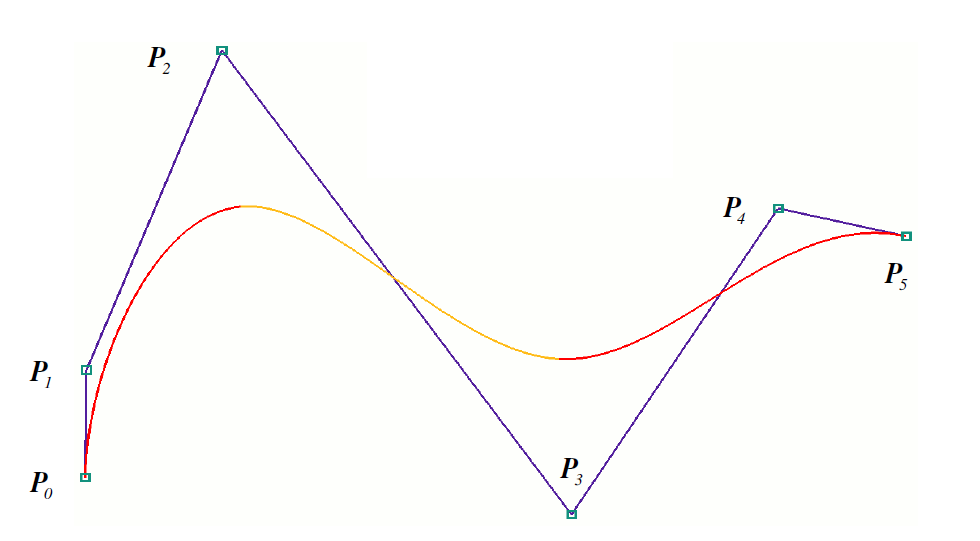
\includegraphics[width=0.75\linewidth]{Bsplines_figure1.png}
\caption{Cubic B-spline with 6 control points.$^{\cite{lockyer2007controlling}}$}
\label{fig:Cubic B-Spline}
\end{figure}

\begin{subsection}{Control points}
In FEM, we need nodes to generate mesh similarly in IGA we require control points which are co-ordinates of the curve. The shape of the curve depends on the control point position and degree of the B-spline. Control points for complex geometries can be download as text file from any design software. 
\end{subsection}

\begin{subsection}{Degree of the B-spline}
The order or degree of B-splines represents the number of control point which influence the position of the curve. This can be clearly seen in  Fig[\ref{fig:B-spline for various degrees}]. The maximum degree of the B-spline curve is one less then the number of control points.

\begin{figure}[h!]
\centering
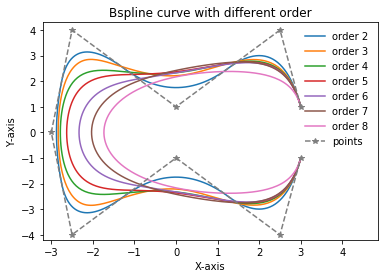
\includegraphics[width=0.9\linewidth]{Bspline_curve_different_order.png}
\caption{B-spline with 9 control points plotted for different degrees.}
\label{fig:B-spline for various degrees}
\end{figure}

\end{subsection}

\begin{subsection}{Generation of Knot vector}
The spacing of knots in the knot vector has a significant effect on the shape of a B-spline curve. In IGA, knot vector is an array of values arranged in ascending order. A knot vector divides the knot span into elements known as patches.


Knot vector ${\displaystyle \xi =\{\xi _{1},\xi _{2},...,\xi _{n+p+1}\}}$,${\displaystyle n}$ is the number of functions, ${\displaystyle p}$ refers to the basis functions degree.

The simplest method of specifying knot vector is by evenly spacing. If the first and the last knots appear ${\displaystyle p+1}$ times, the knot vector is said to be open.As shown in Fig[\ref{fig:B-spline curve of evenly space open clamped knot vector}].


\begin{figure}[h!]
\centering
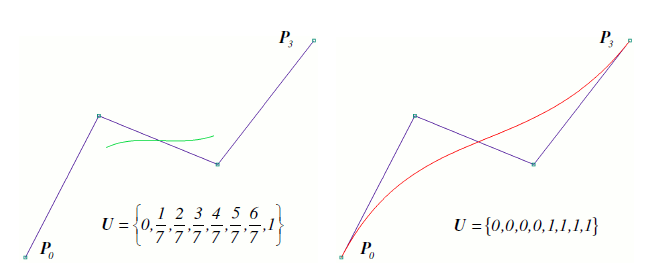
\includegraphics[width=0.75\linewidth]{knot_vector_clamped_unclamped.png}
\caption{B-spline curve of open and clamped knot vector.$^{\cite{lockyer2007controlling}}$}
\label{fig:B-spline curve of evenly space open clamped knot vector}
\end{figure}
\begin{verbatim} 
--------------------------------------------------------------------
def knot_vector(self, n, degree):
        '''
        This function return knot vector based on the number of
        control points and degree of B-spline
        Parameters
        ----------
        control_points : int
            number of points along with weights.
        degree : int
            order of B-splines  0-constant, 1-linear, 2-quadratic
            ,3-cubic.

        Returns
        -------
        knotvector - an array containing knots based on 
        			 control points
        '''
--------------------------------------------------------------------
\end{verbatim}

The function knot vector is implemented as method in Input class.
To run the test case. 
\begin{verbatim} 
------------------------------------------------------------------
(1) pytest test_Inputs.py::test__knotvector_true
------------------------------------------------------------------
\end{verbatim}
The function output is compared with the value obtained from NURBS book $^{\cite{10.5555/265261}}$.


\begin{figure}[h!]
\centering
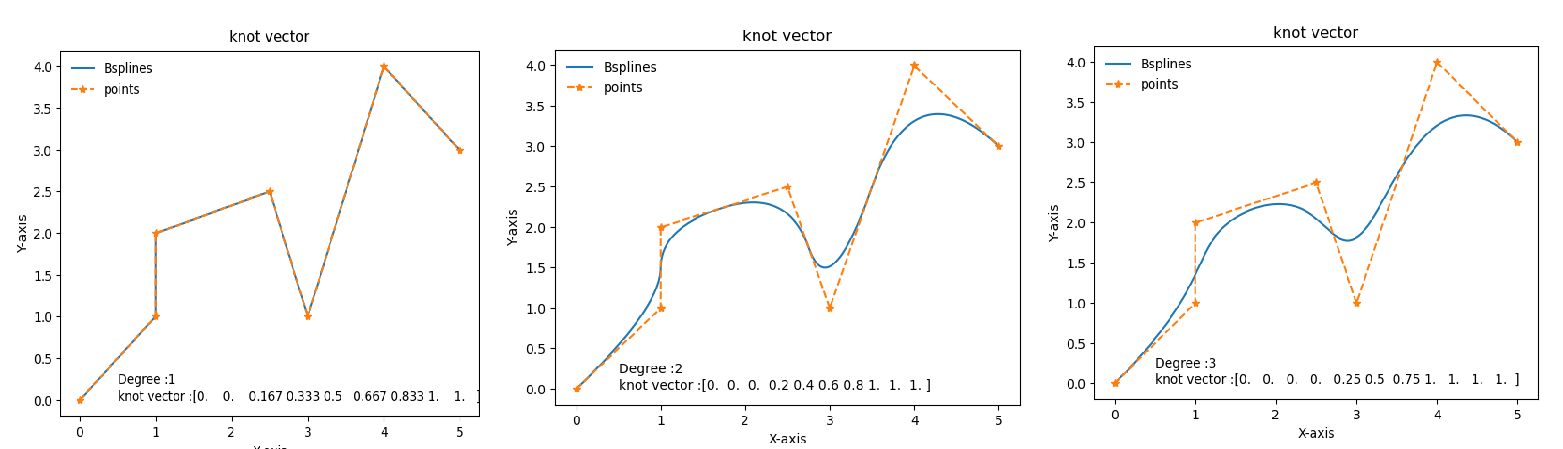
\includegraphics[width=\linewidth]{knot_vector_combined.png}
\caption{Knot vector and B-spline curve change due to change in degree.}
\label{fig:change in knot vector and B-spline curve due to change in degree}
\end{figure}

\end{subsection}
\begin{subsection}{B-spline Basis function}
B-spline basis function is defined as recurrence formula using Cox-de-Boor formula, starting with the zeroth order basis function (p = 0).$^{\cite{NGUYEN201589}}$. 


\begin{equation}\label{Cox-de-Boor formula zero basics}
N_{i, 0}(\xi)=\left\{\begin{array}{ll}
1 & \text { if } \xi_{i} \leq \xi<\xi_{i+1} \\
0 & \text { otherwise }
\end{array}\right.
\end{equation}

and for a polynomial order p greater then one
\begin{equation}\label{Cox-de-Boor formula higher order}
N_{i, p}(\xi)=\frac{\xi-\xi_{i}}{\xi_{i+p}-\xi_{i}} N_{i, p-1}(\xi)+\frac{\xi_{i+p+1}-\xi}{\xi_{i+p+1}-\xi_{i+1}} N_{i+1, p-1}(\xi) .
\end{equation}

\begin{figure}[h!]
\centering
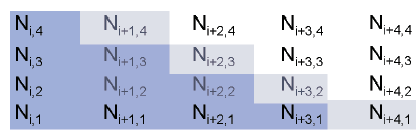
\includegraphics[width=0.75\linewidth]{Bspline_basis_recussive.png}
\caption{B-spline basis dependancy on other basis.$^{\cite{owens2009implementation}}$}
\label{fig:B-spline basis dependancy on other basis}
\end{figure}


B-splines function are not interpolatory i.e, value donot pass through them but the curves are approximated. Fig[\ref{fig:B-spline basis dependancy on other basis}] show how the higher order basis functions depend on lower order basis functions.

 
\begin{verbatim} 
--------------------------------------------------------------------
def bspline_basis(knot_index,degree,U,knotvector):
    '''
    modified version based on Algorthim 2.2 THE NURBS book pg70

    Parameters
    ----------
    knotindex : int 
        DESCRIPTION. The default is ''.

    degree : int
        order of B-splines  0-constant, 1-linear, 2-quadratic, 
        3-cubic
    U : int
            The value whose basis are to be found
    knotvector : array or list
            	list of knot values.
    Returns
    -------
    Basis array of dimension degree+1
        It contains non-zero cox de boor based basis function
            Ex= if degree=2 and knotindex=4 
            basis=[N 2_0, N 3_1, N 4_2]

    '''
--------------------------------------------------------------------
\end{verbatim}
\subsubsection{Properties of B-spline basis function}
%\begin{subsubsection}{Properties of B-spline basis function}

Some properties of B-spline basis function. The values for the test cases are obtained from the NURBS book.$^{\cite{10.5555/265261}}$.
\begin{itemize}
\item They constitute a partition of unity.


\item Each basis function is non-negative over the entire parametric domain

\item They are linearly independent
\end{itemize}
Given below are respective commands to run the test cases
\begin{verbatim} 
------------------------------------------------------------------
(2) pytest test_geometry.py::test__Bspline_basis_sum_equal_to_one_true

(3) pytest test_geometry.py::test__Bspline_basis_all_values_positive_true

(4) pytest test_geometry.py::test__Bspline_basis_equal_true
------------------------------------------------------------------
\end{verbatim}

\subsubsection{Derivatives of B-spline functions}
To implement FEM, we require the derivatives of the basis function. For IGA the first order derivatives are sufficient.

\begin{equation}\label{B-spline Derivative}
\frac{d}{d \xi} N_{i, p}(\xi)=\frac{p}{\xi_{i+p}-\xi_{i}} N_{i, p-1}(\xi)-\frac{p}{\xi_{i+p+1}-\xi_{i+1}} N_{i+1, p-1}(\xi)
\end{equation}  
\begin{verbatim}
---------------------------------------------------------------
def derbspline_basis(knot_index,degree,U,knotvector,order=1):
    """
    Modified version based on the alogorithm A2.3 
    in NURBS Book page no.72
    Parameters
    ----------
    knot_index : integer
                The position of the value U in knotvector
    degree : int
        order of B-splines  0-constant, 1-linear, 2-quadratic,
         3-cubic
    U : int
            The value whose basis are to be found
    knotvector : array or list
            list of knot values.
            
	order :int 
		default :1
		
    Returns
    -------
    Array 
        Derivatives of Basis array of dimension degree+1
        It contains non-zero cox de boor based basis function
            Ex= if degree=2 and knotindex=4 
            der_basis=[N' 2_0, N' 3_1, N' 4_2].
      """
------------------------------------------------------------------
\end{verbatim}

\begin{figure}[h!]
\centering
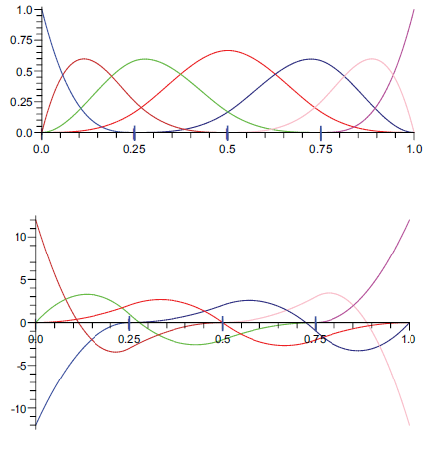
\includegraphics[width=0.75\linewidth]{bspline_function_and_derivative_cubic.png}
\caption{a)Cubic B-spline basis function b) Cubic B-spline derivative function .$^{\cite{10.5555/265261}}$}
\label{fig:Cubic Bspline basis function and it's derivative}
\end{figure}

\paragraph{Properties of B-spline basis function}
%\begin{subsubsection}{Properties of B-spline basis function}
Some properties of derivatives of B-spline basis function. The values for the test cases are obtained from the NURBS book.$^{\cite{10.5555/265261}}$.
 
\begin{itemize}
\item Derivative of basis functions sum upto to zero $\sum_{i=0}^{n}d N_{i, p}(\xi)=0$.

\item They are linearly independent

\end{itemize}
Given below are respective commands to run the test cases.
\begin{verbatim} 
------------------------------------------------------------------
(5) pytest test_geometry.py::test__derbspline_basis_sum_equal_zero_true

(6) pytest test_geometry.py::test__derbspline_basis_equal_true
------------------------------------------------------------------
\end{verbatim}
%\end{subsection}
\end{subsection}


\end{section}


\begin{section}{NURBS (Non-Uniform Rational B-splines) }
B-spline are useful for free-form drawing but lack the flexibility to represent simple geometry like circle and ellipsoid. Therefore NURBS are used which make use of weight functions and have the ability to form exact representation of circles, paraboloids and ellipsoids.

In Fig[\ref{fig:NURBS and B-splines representation and differance}] NURBS with weight equal to one represent B-splines. 

\begin{figure}[h!]
\centering
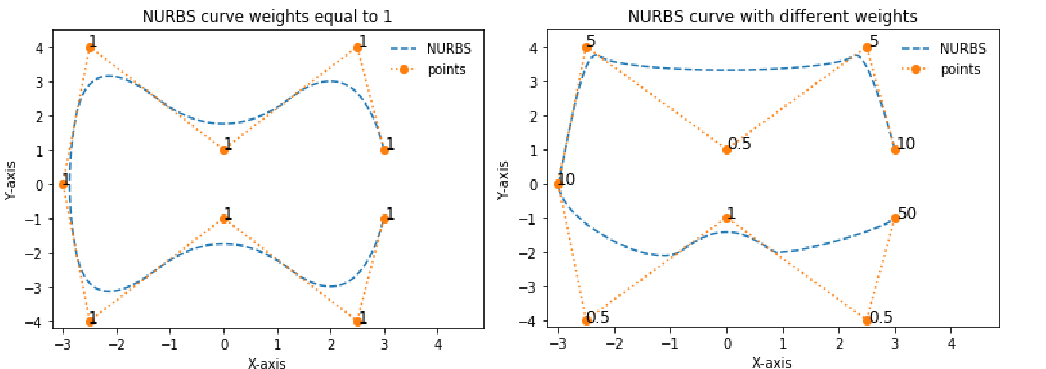
\includegraphics[width=\linewidth]{NURBS_combined_bspline.png}
\caption{a) B-spline b) NURBS}
\label{fig:NURBS and B-splines representation and differance}
\end{figure}

\begin{subsection}{NURBS basis function}
Similar to B-spline basis function, NURBS depend on additional weight parameter.
It is defined as:
\begin{equation}\label{NURBS basis function}
R_{i, p}(\xi)=\frac{N_{i, p}(\xi) w_{i}}{W(\xi)}=\frac{N_{i, p}(\xi) w_{i}}{\sum_{i=1}^{n} N_{\hat{i}, p}(\xi) w_{i}}
\end{equation}

By selecting appropriate weights, we can describe many type of curves.  

\begin{figure}[h!]
\centering
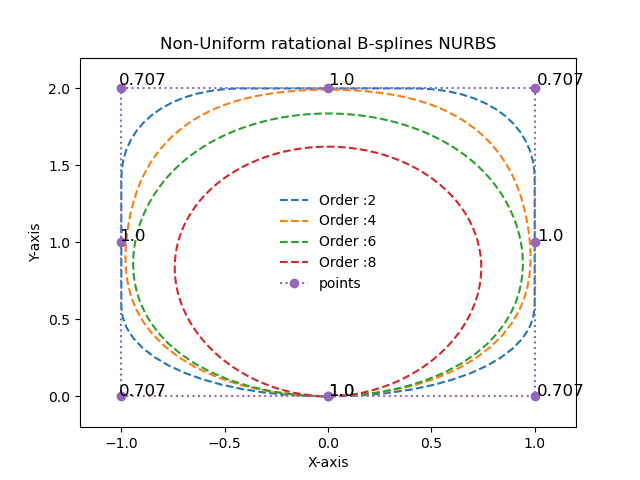
\includegraphics[width=0.85\linewidth]{NURBS_circle.png}
\caption{Circle from NURBS}
\label{fig:NURBS circle for different degree}
\end{figure}

NURBS has to satisfy all properties of B-splines, NURBS are function of B-splines and form superset of them.

\end{subsection}

\begin{subsection}{NURBS derivative function}
The first derivative of a NURBS basis function is computed using the quotient rule as $^{\cite{owens2009implementation}}$

\begin{equation}\label{NURBS derivatives}
\frac{d}{d \xi} R_{i, p}(\xi)=w_{i} \frac{N_{i, p}^{\prime}(\xi) W(\xi)-N_{i, p}(\xi) W^{\prime}(\xi)}{W(\xi)^{2}}
\end{equation}

$\text { where } N_{i, p}^{\prime}(\xi) \equiv \frac{d}{d \xi} N_{i, p}(\xi) \text { and }$
\begin{equation}\label{weights}
W^{\prime}(\xi)=\sum_{\hat{i}=1}^{n} N_{i, p}^{\prime}(\xi) w_{i}^{n}
\end{equation}
\end{subsection}

\begin{subsection}{NURBS volume}
The most important relation required for IGA is the NURBS volume which is the tensor product of NURBS basis in 3 directions.
\begin{equation}\label{NURBS volume}
V(\xi, \eta, \zeta)=\sum_{i=0}^{n} \sum_{j=0}^{m} \sum_{k=0}^{l} R_{i, j, k}^{p, q, r}(\xi, \eta, \zeta) P_{i, j, k}
\end{equation}

\begin{figure}[h!]
\centering
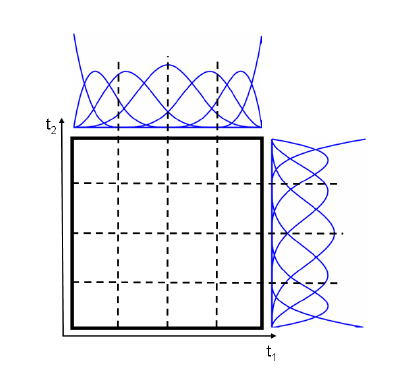
\includegraphics[width=0.75\linewidth]{NURBS_2D_surface.png}
\caption{ NURBS surface.$^{\cite{owens2009implementation}}$}
\label{fig:NURBS surface}
\end{figure}

where the trivariant function is given as
\begin{equation}\label{Trivariant function}
R_{i, j, k}^{p, q, r}(\xi, \eta, \zeta)=\frac{N_{i, p}(\xi) N_{j, q}(\eta) N_{k, r}(\zeta) w_{i, j, k}}{\sum_{i=0}^{n} \sum_{j=0}^{m} \sum_{k=0}^{l} N_{i, p}(\xi) N_{j, q}(\eta) N_{k, r}(\zeta) w_{i, j, k}}
\end{equation}

For easy representation,As shown in fig[\ref{fig:NURBS surface}] a surface is considered. In 2D, Control points form a net and knot vector along t1,t2 form patches. In 3D, knot vector along U,V,W form a patches.

\subsubsection{Derivative of Trivariant basis function}
Derivative of trivariant basis function follow chain rule
\begin{equation}
\frac{\partial R_{i, j,k}^{p, q,r}}{\partial \xi}=\frac{N_{i, p}^{\prime} N_{j, q}N_{k, r} W-N_{i, p} N_{j, q} N_{k, r}W_{\xi}^{\prime}}{W^{2}} w_{i, j}
\end{equation}

\begin{equation}
\frac{\partial R_{i, j,k}^{p, q,r}}{\partial \eta}=\frac{N_{i, p} N_{j, q}^{\prime}N_{k, r} W-N_{i, p} N_{j, q} N_{k, r}W_{\eta}^{\prime}}{W^{2}} w_{i, j}
\end{equation}


\begin{equation}
\frac{\partial R_{i, j,k}^{p, q,r}}{\partial \zeta}=\frac{N_{i, p} N_{j, q}N_{k, r}^{\prime} W-N_{i, p} N_{j, q} N_{k, r}W_{\zeta}^{\prime}}{W^{2}} w_{i, j}
\end{equation}
where
\begin{equation}
W=\sum_{i=0}^{n} \sum_{j=0}^{m}\sum_{k=0}^{l} N_{i, p} N_{j, q} N_{k, r}w_{i, j}
\end{equation}

\begin{equation}
W_{\xi}^{\prime}=\sum_{i=0}^{n} \sum_{j=0}^{m} \sum_{k=0}^{k} N_{i, p}^{\prime} N_{j, q} N_{k, r} w_{i, j}
\end{equation}

\begin{equation}
W_{\eta}^{\prime}=\sum_{i=0}^{n} \sum_{j=0}^{m} \sum_{k=0}^{k} N_{i, p} N_{j, q}^{\prime} N_{k, r} w_{i, j}
\end{equation}

\begin{equation}
W_{\zeta}^{\prime}=\sum_{i=0}^{n} \sum_{j=0}^{m} \sum_{k=0}^{k} N_{i, p} N_{j, q} N_{k, r}^{\prime} w_{i, j}
\end{equation}
\end{subsection}
\begin{verbatim}
------------------------------------------------------------
def trilinear_der(Ux,Uy,Uz,weights,xdegree,xknotvector,ydegree,
					yknotvector,zdegree,zknotvector):
    '''
    

    Parameters
    ----------
    Ux : TYPE
        DESCRIPTION.
    Uy : TYPE
        DESCRIPTION.
    Uz : TYPE
        DESCRIPTION.
    weights : TYPE
        DESCRIPTION.
    xdegree : TYPE, optional
        DESCRIPTION. The default is XI_DEGREE.
    xknotvector : TYPE, optional
        DESCRIPTION. The default is XI_KNOTVECTOR.
    ydegree : TYPE, optional
        DESCRIPTION. The default is ETA_DEGREE.
    yknotvector : TYPE, optional
        DESCRIPTION. The default is ETA_KNOTVECTOR.
    zdegree : TYPE, optional
        DESCRIPTION. The default is ETA_DEGREE.
    zknotvector : TYPE, optional
        DESCRIPTION. The default is ETA_KNOTVECTOR.

    Returns
    -------
    None.
	An array
    '''
------------------------------------------------------------
\end{verbatim}
The values for the test cases are obtained from the NURBS book$^{\cite{10.5555/265261}}$.Given below are respective commands to run the test cases
\begin{verbatim}
-------------------------------------------------------------
(7) pytest test_geometry.py::test__trilinear_der_Basis_sum_equal_to_one_true

(8) pytest test_geometry.py::test__trilinear_der_Basis_less_than_zero_false

(9) pytest test_geometry.py::test__trilinear_der_XI_sum_equal_to_zero_true

(10) pytest test_geometry.py::test__trilinear_der_ETA_sum_equal_to_zero_true

(11) pytest test_geometry.py::test__trilinear_der_NETA_sum_equal_to_zero_true
-------------------------------------------------------------
\end{verbatim}
\end{section}

%%%%%%%%%%%%%%%%
\begin{section}{Background Theory}
\begin{subsection}{Constitutive equation and their weak form}
Based on conservation of linear momentum. The equilibrium equation is given below.
\begin{equation}\label{strong form}
\sigma_{i j, j}+f_{i}=0
\end{equation}
The $\sigma_{i j, j}$ is known as stress tensor and f$_{i}$ is body force vector.\\

The weak form of the equ(\ref{strong form}) can be obtained by using virtual displacment principle and integrated over the domain $\Omega$.

\begin{equation}
\int_{\Omega} \delta u_{i}\left(\sigma_{i j, j}+f_{i}\right) d \Omega=0
\end{equation}
Integration by parts yields
\begin{equation}
\int_{\Gamma}\left(\delta u_{i} \sigma_{i j} n_{j}\right) d \Gamma+\int_{\Omega}\left(f_{i} \delta u_{i}-\delta u_{i, j} \sigma_{i j}\right) d \Omega=0
\end{equation}
where $\Gamma$ is surface integral. based on cauchy's stress formula and kinematic strain relation.
\begin{equation}
T_{i}=\sigma_{i j} n_{j}
\end{equation}
\begin{equation}
\epsilon_{i j}=\left\{\begin{array}{ll}
u_{i, j} & i=j \\
u_{i, j}+u_{j, i} & i \neq j
\end{array}\right.
\end{equation}

Then the weak form is reduced to 
\begin{equation}
\sum_{i}\left[\int_{\Omega}\left(f_{i} \delta u_{i}\right) d \Omega+\int_{\Gamma}\left(T_{i} \delta u_{i}\right) d \Gamma-\int_{\Omega}\left(\delta u_{i, j} \sigma_{i j}\right) d \Omega\right]=0
\end{equation}

\end{subsection}

\begin{subsection}{IGA Formulation}
Similar to FEM, we use Galerkin approximation such that the virtual displacements are given as.
\begin{equation}
\delta u_{i}=\sum_{m=1}^{n} \delta u_{i}^{m} R_{m}
\end{equation}
$\delta u_{i}^{m}$ are the nodal displacements and  R$_{m}$ are the basis functions.
\begin{equation}
\mathbf{R}=\left[\begin{array}{ccccccccc}
R_{1}(\xi, \eta, \zeta) & 0 & 0 & R_{2}(\xi, \eta, \zeta) & 0 & \ldots & R_{n_{c}^{c}}(\xi, \eta, \zeta) & 0 & 0 \\
0 & R_{1}(\xi, \eta, \zeta) & 0 & 0 & R_{2}(\xi, \eta, \zeta) & \ldots & 0 & R_{n_{c p}^{c}}(\xi, \eta, \zeta) & 0 \\
0 & 0 & R_{1}(\xi, \eta, \zeta) & 0 & 0 & R_{2}(\xi, \eta, \zeta) & \ldots & 0 & R_{n_{c p}^{c}}(\xi, \eta, \zeta)
\end{array}\right]
\end{equation}
Degree's of freedom vector q${\alpha}$ is given as 
\begin{equation}
q_{\alpha}=\left[u_{1}^{1}, u_{2}^{1}, u_{3}^{1}, \ldots, u_{1}^{n}, u_{2}^{n}, u_{3}^{n}\right]
\end{equation}
The strains are expressed as 
\begin{equation}
\delta \epsilon_{i j}=\frac{\partial \epsilon_{i j}}{\partial q_{\alpha}} \delta q_{\alpha}
\end{equation}

Then the weak form is expressed as

\begin{equation}
\sum_{\alpha}\left[\sum_{i}\left[\int_{\Omega}\left(f_{i} \frac{\partial u_{i}}{\partial q_{\alpha}}\right) d \Omega+\int_{\Gamma}\left(T_{i} \frac{\partial u_{i}}{\partial q_{\alpha}}\right) d \Gamma-\int_{\Omega}\left(\sigma_{i j} \frac{\partial \epsilon_{i j}}{\partial q_{\alpha}}\right) d \Omega\right]\right]=0
\end{equation}

A strain-displacement matrix is expressed in terms of displacements
and strain via the kinematic relations.
The stress tensor is expressed in terms of displacements by utilizing
kinematic and constitutive relations. The constitutive matrix relates stress and strain.
\begin{equation} \label{BMatrix}
\textbf{B}_{k,\alpha} =
\begin{bmatrix}
R_{1,x} & 0 & 0 & R_{2,x} & 0 & 0 & .... & R_{n_{cp}^e,x} & 0 & 0 \\
0 &R_{1,y} & 0 & 0 & R_{2,y} & 0 & .... & 0 & R_{n_{cp}^e,y} & 0  \\
0 & 0 & R_{1,z} &0 & 0 & R_{2,z} & .... &0 & 0 & R_{n_{cp}^e,z}  \\
R_{1,y} & R_{1,x} & 0 & R_{2,y} & R_{2,x} & 0 & .... & R_{n_{cp}^e,y} &
R_{n_{cp}^e,x} & 0 \\
0 & R_{1,z} & R_{1,y} & 0 & R_{2,z} & R_{2,y} & .... & 0 & R_{n_{cp}^e,z} &
R_{n_{cp}^e,y}\\
R_{1,z} &0 & R_{1,x} & R_{2,z} &0 & R_{2,x} & .... &R_{n_{cp}^e,z} &0
&R_{n_{cp}^e,x}
\end{bmatrix}
\end{equation}
\begin{equation}
\epsilon_{k}=B_{k \alpha} q_{\alpha}
\end{equation}
\begin{equation}
\sigma_{k}=C_{k l} \epsilon_{l}=C_{k l} B_{l \alpha} q_{\alpha}
\end{equation}
The constitutive matrix is calculated based on material properties.
The integral of $\int_{\Omega}\left(B^{T} C B q\right)$ as stiffness matrix (K).
\begin{equation}\label{stiffness matrix}
\int_{\Omega}\left(B^{T} C B q\right) d \Omega=K q
\end{equation}

The force vector is expressed as 
\begin{equation}\label{force vector}
F_{\alpha}=\int_{\Omega} f_{i} \frac{\partial u_{i}}{\partial q_{\alpha}} d \Omega+\int_{\Gamma} T_{i} \frac{\partial u_{i}}{\partial q_{\alpha}} d \Gamma
\end{equation}


\end{subsection}


\begin{subsection}{Topology optimization using IGA}
Topology optimization can be described as binary compliance problem which is use to find a "black and white" layout that minimizes the compliance subjected to volume constrain. There are many frameworks like homogenization method and density-based approach.In our case, the material properties are assumed constant within each element. We implement density-based approach as it restricts the formation of pores and solved the minimum compliance effectively.\\
In density-based approach, the problem is parametrized by the material density distribution. The stiffness tensor are determined using a power-law interpolation function. The power-law implicilty penalizes the intermediate density values to remove pores in structure layout. This penalization method is referred as \textit{ Solid Isotropic Material with Penalization} (SIMP). 

\subsubsection{Solid Isotropic Material with Penalization (SIMP) Method}
SIMP method is a heuristic relation
between element density  and element Young’s modulus. It given by 
\begin{equation}
\left.\left.E_{i}=E_{i}\left(x_{i}\right)=x_{i}^{p} E_{0}, \quad x_{i} \in\right] 0,1\right]
\end{equation}
the element density is given as
\begin{equation}
x_i=\left\{\begin{array}{lll}
1 & \text { if } & \mathbf{x} \in \Omega_{s} \\
0 & \text { if } & \mathbf{x} \in \Omega \backslash \Omega_{s}
\end{array}\right.
\end{equation}
The element densities are approximated by the NURBS basis functions over a patch.
\begin{equation}
x_{r, s}=\sum_{i=0}^{n_{1}} \sum_{i=1}^{n_{2}} R_{i, j}(r, s) x^{p}_{i j}
\end{equation}

where E$_0$ is the elastic modulus of material, E$_{min}$ is the minimum elastic modulus of the void region which prevents stiffness matrix singularity. \textbf{P} is the penalization factor introduced to ensure black and white layout.A modified SIMP method is given below.
\begin{equation}
\mathrm{E}_{i}=\mathrm{E}_{i}\left(x_{i}\right)=\mathrm{E}_{\min }+x_{i}^{p}\left(\mathrm{E}_{0}-\mathrm{E}_{\min }\right), \quad x_{i} \in[0,1]
\end{equation}
\textbf{Advantages of modified SIMP method}
\begin{enumerate}
\item Independency of the problem on minimum value of material's elastic modulus and the penalization power.
\end{enumerate}

\subsubsection{Minimum Compliance formulation}

The main objective of minimum compliance formulation is to find material density distribution that minimizes deformation for prescribed support and loading condition.
The compliance is given as,
\begin{equation}
c(\overline{\mathbf{x}})=\mathbf{F}^{\mathrm{T}} \mathbf{U}(\overline{\mathbf{x}})
\end{equation}
where F is the vector of nodal forces and U(x) is the vector
of nodal displacements.\\
The mathematical formulation of the optimization problem reads as follows:
\begin{equation}
\text { minimize }: c(x)=U^{T} K U=\sum_{e=1}^{N} E_{e}\left(x_{e}\right) u_{e}^{T} k_{0} u_{e}
\end{equation}

\begin{equation}
\text { subject to }:\left\{\begin{array}{l}
\frac{V(x)}{V_{0}}=f \\
K U=F \\
0 \leq x \leq 1
\end{array}\right.
\end{equation}

Where C is compliance, k$_0$ is the element stiffness matrix, N number of elements, V(x) and V$_0$ are the material volume and design volume. \textit{f} is the prescribed volume fraction.\\
The derivatives of the compliance is 
\begin{equation}
\frac{\partial c(\overline{\mathbf{x}})}{\partial x_{e}}=\sum_{i \in N_{e}} \frac{\partial c(\overline{\mathbf{x}})}{\partial \tilde{x}_{i}} \frac{\partial \tilde{x}_{i}}{\partial x_{e}}
\end{equation}

\begin{equation}
\begin{aligned}
\frac{\partial c(\overline{\mathbf{x}})}{\partial \tilde{\mathbf{x}}_{i}} &=\mathbf{F}^{\mathrm{T}} \frac{\partial \mathbf{U}(\overline{\mathbf{x}})}{\partial \tilde{\mathbf{x}}_{i}} \\
&=\mathbf{U}(\overline{\mathbf{x}})^{\mathrm{T}} \mathbf{K}(\overline{\mathbf{x}}) \frac{\partial \mathbf{U}(\overline{\mathbf{x}})}{\partial \overline{\mathbf{x}}_{i}}
\end{aligned}
\end{equation}
\begin{equation}\label{KU}
\mathbf{K}(\tilde{\mathbf{x}}) \mathbf{U}(\overline{\mathbf{x}})=\mathbf{F}
\end{equation}
The above equation(\ref{KU}) is derivatived with respect to element density.
\begin{equation}
\frac{\partial \mathbf{K}(\overline{\mathbf{x}})}{\partial \overline{\mathbf{x}}_{i}} \mathbf{U}(\overline{\mathbf{x}})+\mathbf{K}(\overline{\mathbf{x}}) \frac{\partial \mathbf{U}(\tilde{\mathbf{x}})}{\partial \tilde{\mathbf{x}}_{i}}=\mathbf{0}
\end{equation}
which yields,
\begin{equation}
\frac{\partial \mathbf{U}(\tilde{\mathbf{x}})}{\partial \overline{\mathbf{x}}_{i}}=-\mathbf{K}(\tilde{\mathbf{x}})^{-1} \frac{\partial \mathbf{K}(\overline{\mathbf{x}})}{\partial \tilde{\mathbf{x}}_{i}} \mathbf{U}(\overline{\mathbf{x}})
\end{equation}

On substitution, the objective function is obtained.\\
Compliance constrain:
\begin{equation}
\frac{\partial c(\tilde{\mathbf{x}})}{\partial \tilde{\mathbf{x}}_{i}}=-\mathbf{u}_{i}(\tilde{\mathbf{x}})^{\mathrm{T}}\left[\mid p \tilde{\mathrm{X}}_{i}^{p-1}\left(\mathrm{E}_{0}-\mathrm{E}_{\min }\right) \mathbf{k}_{i}^{0}\right] \mathbf{u}_{i}(\overline{\mathbf{x}})
\end{equation}

Volume constrain:
\begin{equation}
\frac{\partial v(\tilde{\mathbf{x}})}{\partial x_{e}}=\sum_{i \in N_{e}} \frac{\partial v(\overline{\mathbf{x}})}{\partial \tilde{x}_{i}} \frac{\partial \bar{x}_{i}}{\partial x_{e}}
\end{equation}

The objective function are obtained, we require optimization algorithm to solve them to get minimization. 
\subsubsection{Sensitivity}
To ensure that topology optimization problem would exist and avoid the formation of checker board pattern or pores in the design. This can be achieved by applying filter or sensitivity to objective function like compliance and volume constrains.\\
Basic filter function is defined as
\begin{equation}
\bar{x}_{e}=\frac{\sum_{i \in N_{c}} H_{e i} x_{i}}{\sum_{i \in N_{c}} H_{e i}}
\end{equation}
where H$_{e i}$ is the weight factor given as.
 \begin{equation}
H_{e i}=\max \left(0, r_{\min }-\Delta(e, i)\right)
\end{equation}
Based on filter radius r$_{min}$, we calculate the center-to-center distance between elements $\Delta(e, i)$. \\
The sensitivity for
the objective function c and the material volume V with respect to design variable x$_i$.
is now given as:
\begin{equation}
\frac{d c}{d x_{j}}=\sum_{e \in N_{j}} \frac{1}{\sum_{i \in N_{c}} H_{e i}} H_{j e} \frac{d c}{\bar{x}_{e}}
\end{equation}
\begin{equation}
\frac{d V}{d x_{j}}=\sum_{\epsilon \in N_{j}} \frac{1}{\sum_{i \in N_{e}} H_{e i}} H_{j e} \frac{d V}{\tilde{x}_{e}}
\end{equation}
\begin{verbatim}
----------------------------------------------------------------------

def Knearestneighbours(rmin,nelx,nely,nelz):
    '''
    function used to generate weight factor from the given parameters

    Parameters
    ----------
    rmin : float
        minimum radius to describe the radius of the filter.
    nelx : int
        No of elements in x.
    nely : int
        No of elements in y.
    nelz : int
        No of elements in z.

    Returns
    -------
    H : numpy array
        An array of weight function for each element.
    DH : numpy array
        sum of all weight function saved as single array .

    '''
----------------------------------------------------------------------
\end{verbatim}
\subsubsection{Optimality criteria method}
To solve structural optimization problem using optimality criteria (OC) method.In OC method, the constrains  0 < x < 1 is inactive. The convergence can able be achieved if the KKT condition are satisfied. 
\begin{equation}
\frac{\partial c(\overline{\mathbf{x}})}{\partial x_{e}}+\lambda \frac{\partial v(\overline{\mathbf{x}})}{\partial x_{e}}=0
\end{equation}

The implementation of OC update scheme is given below.
\begin{equation}
x_{e}^{\text {new }}=\left\{\begin{array}{l}
\max \left(0, x_{e}-m\right), \text { if } x_{e} B_{e}^{\eta} \leq \max \left(0, x_{e}-m\right) \\
\min \left(1, x_{e}+m\right), \text { if } x_{e} B_{e}^{\eta} \geq \min \left(1, x_{e}-m\right) \\
x_{e} B_{e}^{\eta}, \text { otherwise }
\end{array}\right.
\end{equation}
where m is move limit and $\eta$ is numerical damping coefficient and optimality condition B$_e$ is obtained from equation(\ref{OC_Be}).
\begin{equation}\label{OC_Be}
B_{e}=-\frac{\partial c(\overline{\mathbf{x}})}{\partial x_{e}}\left(\lambda \frac{\partial v(\overline{\mathbf{x}})}{\partial x_{e}}\right)^{-1}
\end{equation}
The unknown value $\lambda$ is the lagrangian multiplier which is obtained by root finding algorithm such as bi-section method.\\

\textbf{Bi-section method}
\begin{enumerate}
\item Choose lower(l) and upper(u) bound values.
\item Compute midpoint m=(l+u)/2 and calculate f(m)
\item Determination of next subinterval based on sign of the product f(l)x f(m) and f(u)x f(m)
\item Repeat till tolerance is achieved.
\end{enumerate}

Test command to check the implementation of OC for simple function and quadratic function.
\begin{verbatim}
----------------------------------------------------------------------
pytest test_optimization.py::test__optimality_criteria_simple_function

pytest test_optimization.py::test__optimality_criteria_quadratic_function

----------------------------------------------------------------------
\end{verbatim}




\subsubsection{Method of moving Asymptotes }

Moving Asymptotes is a gradient based optimization algorithm.
MMA subproblem is given as
\begin{equation}
\operatorname{minimize} \quad \tilde{f}_{0}^{(k)}(\mathrm{x})+a_{0} z+\sum_{i=1}^{m}\left(c_{i} y_{i}+\frac{1}{2} d_{i} y_{i}^{2}\right)
\end{equation}

%\begin{equation}
%\begin{array}{lll}
%\text { subject to } & \tilde{f}_{i}^{(k)}%(\mathrm{x})-a_{i} z-y_{i} \leq 0, & i=1, \ldots, m \\
%& \alpha_{j}^{(k)} \leq x_{j} \leq \beta_{j}^{(k)}, & j=1, \ldots, n \\
%& y_{i} \geq 0, & i=1, \ldots, m \\
%& z \geq 0 & &
%\end{array}
%\end{equation}

An approximate function is build to satisfy the above problem

\begin{equation}
\tilde{f}_{i}^{(k)}(\mathrm{x})=\sum_{j=1}^{n}\left(\frac{p_{i j}^{(k)}}{u_{j}^{(k)}-x_{j}}+\frac{q_{i j}^{(k)}}{x_{j}-l_{j}^{(k)}}\right)+r_{i}^{(k)}, \quad i=0,1, \ldots, m
\end{equation}
where p$_{i j}$ and q$_{i j}$ are given as
\begin{equation}
p_{i j}^{(k)}=\left(u_{j}^{(k)}-x_{j}^{(k)}\right)^{2}\left(1.001\left(\frac{\partial f_{i}}{\partial x_{j}}\left(\mathrm{x}^{(k)}\right)\right)^{+}+0.001\left(\frac{\partial f_{i}}{\partial x_{j}}\left(\mathrm{x}^{(k)}\right)\right)^{-}+\frac{10^{-5}}{x_{j}^{\max }-x_{j}^{\min }}\right)
\end{equation}
\begin{equation}
q_{i j}^{(k)}=\left(x_{j}^{(k)}-l_{j}^{(k)}\right)^{2}\left(0.001\left(\frac{\partial f_{i}}{\partial x_{j}}\left(\mathrm{x}^{(k)}\right)\right)^{+}+1.001\left(\frac{\partial f_{i}}{\partial x_{j}}\left(\mathrm{x}^{(k)}\right)\right)^{-}+\frac{10^{-5}}{x_{j}^{\max }-x_{j}^{\min }}\right)
\end{equation}
\begin{equation}
r_{i}^{(k)}=f_{i}\left(\mathrm{x}^{(k)}\right)-\sum_{j=1}^{n}\left(\frac{p_{i j}^{(k)}}{u_{j}^{(k)}-x_{j}^{(k)}}+\frac{q_{i j}^{(k)}}{x_{j}^{(k)}-l_{j}^{(k)}}\right)
\end{equation}

The lower and upper bound are formulated as below
\begin{equation}
\alpha_{j}^{(k)}=\max \left\{x_{j}^{\min }, \quad l_{j}^{(k)}+0.1\left(x_{j}^{(k)}-l_{j}^{(k)}\right), \quad x_{j}^{(k)}-0.5\left(x_{j}^{\max }-x_{j}^{\min }\right)\right\}
\end{equation}

\begin{equation}
\beta_{j}^{(k)}=\min \left\{x_{j}^{\max }, u_{j}^{(k)}-0.1\left(u_{j}^{(k)}-x_{j}^{(k)}\right), \quad x_{j}^{(k)}+0.5\left(x_{j}^{\max }-x_{j}^{\min }\right)\right\}
\end{equation}

The lower and Upper Asymptotes are calculated using the below relation \\
For iteration less then 3:
\begin{equation}
\begin{aligned}
l_{j}^{(k)} &=x_{j}^{(k)}-0.5\left(x_{j}^{\max }-x_{j}^{\min }\right) \\
u_{j}^{(k)} &=x_{j}^{(k)}+0.5\left(x_{j}^{\max }-x_{j}^{\min }\right)
\end{aligned}
\end{equation}
For iteration greater then 3:
\begin{equation}
\begin{aligned}
l_{j}^{(k)} &=x_{j}^{(k)}-\gamma_{j}^{(k)}\left(x_{j}^{(k-1)}-l_{j}^{(k-1)}\right) \\
u_{j}^{(k)} &=x_{j}^{(k)}+\gamma_{j}^{(k)}\left(u_{j}^{(k-1)}-x_{j}^{(k-1)}\right),
\end{aligned}
\end{equation}
where $\gamma$ is 
\begin{equation}
\gamma_{j}^{(k)}=\left\{\begin{array}{cl}
0.7 & \text { if }\left(x_{j}^{(k)}-x_{j}^{(k-1)}\right)\left(x_{j}^{(k-1)}-x_{j}^{(k-2)}\right)<0 \\
1.2 & \text { if }\left(x_{j}^{(k)}-x_{j}^{(k-1)}\right)\left(x_{j}^{(k-1)}-x_{j}^{(k-2)}\right)>0 \\
1 & \text { if }\left(x_{j}^{(k)}-x_{j}^{(k-1)}\right)\left(x_{j}^{(k-1)}-x_{j}^{(k-2)}\right)=0
\end{array}\right.
\end{equation}\\
\textbf{ Primal-dual method for solving the Moving Asymptotes method}\\

Prime-dual method is part of active set strategy and constrained based non-linear optimization algorithm.It is gradient based method and used Newton Raphson to solve equ(\ref{Lag})
To satisfy constrained problem, we build a Lagrangian function.
\begin{equation}\label{Lag}
\begin{aligned}
L=& \psi(x, \lambda)+\left(a_{0}-\zeta\right) z+\sum_{j=1}^{n}\left(\xi_{j}\left(\alpha_{j}-x_{j}\right)+\eta_{j}\left(x_{j}-\beta_{j}\right)\right)+\\
&+\sum_{i=1}^{m}\left(c_{i} y_{i}+\frac{1}{2} d_{i} y_{i}^{2}-\lambda_{i} a_{i} z-\lambda_{i} y_{i}-\lambda_{i} b_{i}-\mu_{i} y_{i}\right)
\end{aligned}
\end{equation}\\
ALGORTHIM \\


Test command to check the implementation of MMA with quadratic equation and KKT condition provided in literature.[citition]
\begin{verbatim}
----------------------------------------------------------------------
pytest test_optimization.py::test__MMA_literature_equation
----------------------------------------------------------------------
\end{verbatim}

\end{subsection}
\end{section}



\begin{section}{IGTO implementation}
In FEM, we use Lagrangian basis function to discretised both geometry and displacement in iso-parametric method. Even IGA can be iso-parametric formulation.Similar to FEM, IGA can be divided into sub programs

\begin{itemize}
\item Pre-Processing

\item Processing

\item Post-Processing

\end{itemize}
\begin{figure}[h!]
\centering
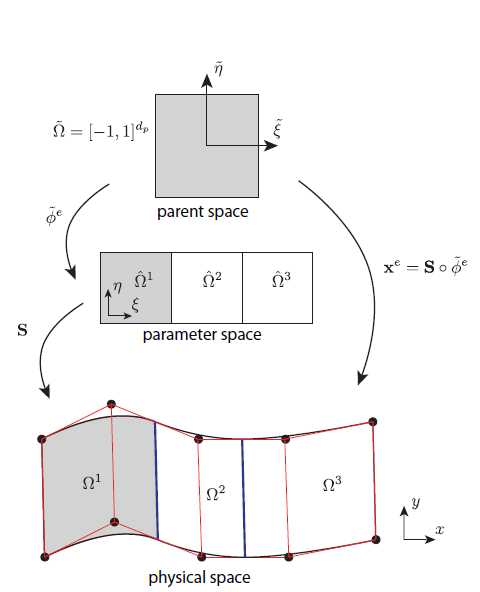
\includegraphics[width=0.45\linewidth]{relevant_spaces.png}
\caption{ Relevant spaces.$^{\cite{NGUYEN201589}}$}
\label{fig:Relevant spaces}
\end{figure}

\begin{subsection}{Relevant spaces}
In FEM, there are parent and unit space. The core concepts in IGA are the outlining the relevant spaces. As shown in fig[\ref{fig:Relevant spaces}]

\begin{enumerate}
\item \textbf{Parent space} 
\\ This space is also known as unit space. The parent space is defined over the interval $\Omega$=[-1,1].This required to implement numerical integration such as gauss quadrature.

\item \textbf{Parameter space}
\\ This space also referred as pre-image of NURBS mapping is formed by using non-zero intervals of knot vectors. In parametric space, the shapes in physical space are normalized. Due to normalization the domain is defined over   $\Omega$=[0,1].
\item \textbf{Physical space}
\\ Physical space is associated with co-ordinate system. NURBS is defined by control points and weights.

\end{enumerate}

\end{subsection}

\begin{subsection}{Pre-processing}
In pre-processing state, the geometry has to be defined.

\subsubsection{Generation of NURBS parameters}
Along with physical parameters like length, breath, width, number of elements along x(nx), number of elements along y(ny), number of elements along z(nz), order along x (xidegree),order along y (etadegree) and order along z (netadegree). We require NURBS parameters like control points and knot vectors to represent geometry. 

A python class is defined to generate NURBS parameters which is given below.
\begin{verbatim}
------------------------------------------------------------

class Inputs():
    '''
    A geometry class with NURBS parameter as the method
    Methods:
        crtpts_coordinates : generate control points along with weights 

        knot_vector :generates knot vector  based on control points 
        generated from crtpts_coordinates and degree

        knotconnect : other parameter required for 
        assembly like span, unique knots are .
        
    '''

    def __init__(self, length=1, height=1, width=1, nx=1, ny=1, nz=1, 
    xidegree=1, etadegree=1, netadegree=1)
------------------------------------------------------------

\end{verbatim}
 "Rhino" a commerical software can be to generate exact parametric values for complex NURBS geometry.
Test cases to check NURBS parameters generated through Inputs class.
\begin{verbatim}
------------------------------------------------------------
(12) pytest test_Inputs.py::test__controlpoints_coordinates_true

(13) pytest test_Inputs.py::test__knotconnect_span_true

------------------------------------------------------------
\end{verbatim}

\subsubsection{Assembly of Geometry}
In IGA, discrization of global geometry into smaller patches is done through assembly array. The assembly array would require a)control points, b)knot vector, c) weights .

The following are the function required to generate a assembly array.\\

1.\textbf{ Element order}\\
A function which generates a 3D array which contains the positions of the elements.


2.\textbf{ knot connectivity}\\
An array which contains the length of each element expressed in the form of knot points.

3.\textbf{ Control point assembly}\\
An array which contains the control points of the element based on the degree and knot connectivity and element order.
 
Number of control points in each element is give as n$^{cp}$=(p+1)*(q+1)*(r+1).
For number of elements 2,1,1 respectively in x,y,z direction with order equal to one, n$^{cp}$=8. The control point array should be as shown in fig[\ref{fig:Control point assembly and node numbering}].
 
\begin{figure}[h!]
\centering
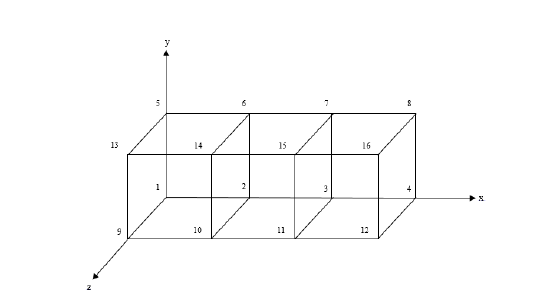
\includegraphics[width=\linewidth]{element numbering.png}
\caption{Control point assembly and node numbering}
\label{fig:Control point assembly and node numbering}
\end{figure}
\begin{verbatim}
------------------------------------------------------------

def controlpointassembly(n,p,q,nU,nV,nW,xdegree,ydegree,zdegree,
knotconnectivityU,knotconnectivityV,knotconnectivityW):# 
    '''
    Inputs:
    n,p,q : int
    	knot points in xi,eta,neta direction
    nU,nV,nW :int
    	number of element in x,y,z direction	
    xdegree,ydegree,zdegree :int
       degree of the NURBS along xi,eta,neta
    knotconnectivityU,knotconnectivityV,knotconnectivityW    
    :int
    
    outputs:
    element assembly : narray
    		consist of control points of the elements
    
    '''
    elements_assembly=np.zeros(((nU*nV*nW),
    	(xdegree+1)*(ydegree+1)*(zdegree+1)))
    elements_order=elementorder(n,p,q)
    a=0 
    for i in range(nW):
        for j in range(nV):
            for k in range(nU):
                c=0
                for l in range(len(knotconnectivityW[i,:])):
                    for m in range(len(knotconnectivityV[j,:])):
                        for n in range(len(knotconnectivityU[k,:])):
                    elements_assembly[a,c]=elements_order[
                    knotconnectivityU[k,n],
				                            			knotconnectivityW[i,l], 
                            									knotconnectivityV[j,m]]
                            c+=1
                a+=1         
    elements_assembly=elements_assembly.astype(int)
    return elements_assembly.

    '''
------------------------------------------------------------
\end{verbatim}



Following are test commands to check the assembly matrix for different values and order
\begin{verbatim}
------------------------------------------------------------
(14) pytest test_geometry.py::test__single_element_Assembly

(15) pytest test_geometry.py::test__element_Assembly_C0_continuity

(16) pytest test_geometry.py::test__single_element_Assembly_C1_continuity_along_x
------------------------------------------------------------
\end{verbatim}


\subsubsection{Boundary conditions}
Implementation of Dirichlet boundary condition for homogeneous case is quite easy as the control points are on the surface and the corresponding control points can be equated to zero. For inhomogeneous case, method like least square have to be implemented which is not in scope of this project.\\
Boundary condition are implemented in the form a python switch class depending on option respective BC are applied, we get fixed control point nodes and load control point nodes. Give below 
\begin{verbatim}
------------------------------------------------------------
class BC_Switcher(object):
	'''
	A python switch class'
	Methods
	 based on option 
	Ex 0 -cantilever beam with load at the end
	INPUTS:
	option
	 CONTROL_POINTS : numpy array
	 Length :float
	 height :float
	 width  :float
	 
	OUTPUTS:
	 fixed nodes: numpy array
	 load nodes : numpy array
	 
    def __init__(self,CONTROL_POINTS,length,height,width,bc_disp):
        self.CONTROL_POINTS=CONTROL_POINTS
        self.length=length
        self.width=width
        self.height=height
        self.bc_disp=bc_disp
-----------------------------------------------------------------------
\end{verbatim}  
\end{subsection}

\begin{subsection}{Processing}
We need to compute global stiffness matrix \textbf{K} and global force vector \textbf{F}. For this, we requires the derivatives of trilinear basis function which is used to formulate jacobian. A numerical integration scheme is employed to solve volume integrals along with mapping physical space to parent space.  

\subsubsection{Mapping relevant spaces}

The use of NURBS basis introduces a parametric space which needs additional mapping from physical to parameteric space and parameteric space to parent space.As shown in fig[\ref{fig:Relevant spaces}]
\paragraph{}
1. \textbf{ Mapping from physical space to parameter space}
\\ The associated Jacobian is represented as $\mathbf{J}_{1}$ and is computed as below.
\begin{equation}
\mathbf{J}_{1}=\left[\begin{array}{lll}
\frac{\partial x}{\partial \xi} & \frac{\partial x}{\partial \eta} & \frac{\partial x}{\partial \zeta} \\
\frac{\partial y}{\partial \xi} & \frac{\partial y}{\partial \eta} & \frac{\partial y}{\partial \zeta} \\
\frac{\partial z}{\partial \xi} & \frac{\partial z}{\partial \eta} & \frac{\partial z}{\partial \zeta}
\end{array}\right]
\end{equation}
The component of the Jacobian 1 are given below
\begin{equation}\label{J1}
\begin{array}{lll}
\frac{\partial x}{\partial \xi}=\sum_{k=1}^{n_{c p}^{e}} \frac{\partial \mathbf{R}_{k}}{\partial \xi} x_{i} & \frac{\partial x}{\partial \eta}=\sum_{k=1}^{n_{c p}^{e}} \frac{\partial \mathbf{R}_{k}}{\partial \eta} x_{i} & \frac{\partial x}{\partial \zeta}=\sum_{k=1}^{n_{c p}^{e}} \frac{\partial \mathbf{R}_{k}}{\partial \zeta} x_{i} \\
\frac{\partial y}{\partial \xi}=\sum_{k=1}^{n_{c p}^{e}} \frac{\partial \mathbf{R}_{k}}{\partial \xi} y_{i} & \frac{\partial y}{\partial \eta}=\sum_{k=1}^{n_{c p}^{e}} \frac{\partial \mathbf{R}_{k}}{\partial \eta} y_{i} &\frac{\partial y}{\partial \zeta}=\sum_{k=1}^{n_{c p}^{e}} \frac{\partial \mathbf{R}_{k}}{\partial \zeta} y_{i}\\
\frac{\partial z}{\partial \xi}=\sum_{k=1}^{n_{c p}^{e}} \frac{\partial \mathbf{R}_{k}}{\partial \xi} z_{i} & \frac{\partial z}{\partial \eta}=\sum_{k=1}^{n_{c p}^{e}} \frac{\partial \mathbf{R}_{k}}{\partial \eta} z_{i} &\frac{\partial z}{\partial \zeta}=\sum_{k=1}^{n_{c p}^{e}} \frac{\partial \mathbf{R}_{k}}{\partial \zeta} z_{i}\\
\end{array}
\end{equation}
components of $\mathbf{J}_{1}$ can be obtained through derivatives of trilinear basis function. 

2. \textbf{ Mapping from parameter space to parent space}
\\ The associated Jacobian is represented as $\mathbf{J}_{2}$ and is computed as below. The $\bar{\xi}$,$\bar{\eta}$,$\bar{\zeta}$ are the gauss quadrature and $\xi_{i+1},\xi_{i}$  are the knot values of that element.
\begin{equation}
\xi=\frac{1}{2}\left[\left(\xi_{i+1}-\xi_{i}\right) \bar{\xi}+\left(\xi_{i+1}+\xi_{i}\right)\right]
\end{equation}
\begin{equation}
\eta=\frac{1}{2}\left[\left(\eta_{i+1}-\eta_{i}\right) \bar{\eta}+\left(\eta_{i+1}+\eta_{i}\right)\right]
\end{equation}

\begin{equation}
\zeta=\frac{1}{2}\left[\left(\zeta_{i+1}-\zeta_{i}\right) \bar{\zeta}+\left(\zeta_{i+1}+\eta_{i}\right)\right]
\end{equation}
The determinent of Jacobian 2 is calculated as shown below.
\begin{equation}\label{J2}
\mathbf{J}_{2}=\frac{\partial \xi}{\partial \bar{\xi}} \frac{\partial \eta}{\partial \bar{\eta}} \frac{\partial \zeta}{\partial \bar{\zeta}}
\end{equation}
Below are the test cases to check the functioning of the Jacobian
\begin{verbatim}
-----------------------------------------------------------------------
(17) pytest test_element_routine.py::test__unit_to_parametric_space_true

(18) pytest test_element_routine.py::test__Jacobian_patch_testing_rotation
-----------------------------------------------------------------------
\end{verbatim}
\subsubsection{Building global stiffness matrix}
From the relation \ref{stiffness matrix}, the element stiffness matrix as below.
\begin{equation}
K^{(e)}=\int_{-1}^{1} \int_{-1}^{1} \int_{-1}^{1} B^{T} C B|J| d \bar{\Omega}_{e}
\end{equation}
Where J =J${_1}$*J${_2}$ obtained from the relation in (\ref{J1}) and (\ref{J2}).\\
Since strain-displacement matrix is a function of derivatives in global co-ordinates and gauss quadrature can be applied only in normalized co-ordinate system. The below relation transform normalized derivatives to co-ordinate derivatives using Jacobian.
\begin{equation}
\frac{\partial R_{m}}{\partial x_{i}}=\frac{\partial \xi_{j}}{\partial x_{i}} \frac{\partial R_{m}}{\partial \xi_{j}}=J_{i j}^{-1} \frac{\partial R_{m}}{\partial \xi_{j}}
\end{equation}
\begin{verbatim}
-----------------------------------------------------------------------
\end{verbatim}
\textbf{Element routine procedure}:\\
1. Loop over elements, $e=1, \ldots,$ nel\\
(a) Determine the co-ordinates of the element using control point assemby matrix\\
(b)  Determine NURBS coordinates $\left[\xi_{i}, \xi_{i+1}\right] \times\left[\eta_{j}, \eta_{j+1}\right] \times\left[\zeta_{j}, \zeta_{j+1}\right]$ using knotspan U,V,W.\\
(c) $\mathbf{K}_{e}=\mathbf{0}$\\
(d) Loop over Gauss points, $\left\{\bar{\xi}_{j}, \bar{w}_{j}\right\} \quad j=1,2, \ldots, n_{g p}$\\
i. Compute $\xi$, $\eta$, $\zeta$   corresponding to $\bar{\xi}_{j}$, $\bar{\eta}_{j}$ and  $\bar{\zeta}_{j}$  \\
ii. Compute $\left|J_{2}\right|$ \\
iii. Compute derivatives of shape functions R at $\xi$,$\eta$ and $\zeta$ from triliniear basis function.\\
iv. Compute $\mathbf{J}_{1}$ using , $\mathbf{R}_{, k}$ and $\mathbf{R}_{, \eta}$ .\\
v. Compute Jacobian inverse $\mathbf{J}_{1}^{-1}$ and determinant $\left|J_{1}\right|$.\\
vi. Compute derivatives of shape functions $\mathbf{R}_{\mathbf{x} \mathbf{x}}=\left[\mathbf{R}_{, \xi} \mathbf{R}_{, \eta}\right] \mathbf{J}_{1}^{-1}$ \\
vii. Use $\mathbf{R}_{, \mathbf{x}}$ to build the strain-displacement matrix $\mathbf{B}$\\ viii. Compute $\mathbf{K}_{e}=\mathbf{K}_{e}+\bar{w}_{j}\left|J_{2} \| J_{1}\right| \mathbf{B}^{\mathrm{T}} \mathbf{D B}$.\\
(f) End loop over Gauss points.\\
(g) Assemble $\mathbf{K}_{e}: \mathbf{K}(\operatorname{sctr} B, \operatorname{sctr} B)=\mathbf{K}(\operatorname{sctr} B, \operatorname{sctr} B)+\mathbf{K}_{e}$.\\
2. End loop over elements.
\begin{verbatim}
-----------------------------------------------------------------------
\end{verbatim}
The above procedure is performed using the following python function.1) gauss quadrature, 2) Jacobian, 3) strain displacement, 4) Compliance matrix, 5) element routine and 6) assemble.

Test commands to check gauss quadrature and global stiffness matrix generated from element routine.
\begin{verbatim}
-----------------------------------------------------------------------
(19) pytest test_element_routine.py::test__gauss_quadrature_1point_true

(20) pytest test_element_routine.py::test__stiffness_matrix_singularity
-----------------------------------------------------------------------
\end{verbatim}

\subsubsection{Topology optimization}
Using SIMP method, the element stiffness matrix is interpolated as,
\begin{equation}
k_{e}\left(\tilde{x}_{e}\right)=E_{e}\left(\tilde{x}_{e}\right) k_{e}^{0}
\end{equation}
where k$_{e}^{0}$ is given as,
\begin{equation}
k{_e}^{0}=\int_{-1}^{1} \int_{-1}^{1} \int_{-1}^{1} B^{T} C^{0} B|J| d \bar{\Omega}_{e}
\end{equation}
On substitution, we get,
 
\begin{equation}
\boldsymbol{K}_{e}=\sum_{j}\left(E_{\min }+\tilde{\rho}\left(\boldsymbol{x}_{j}^{q}\right)^{p}\left(E_{0}-E_{\min }\right)\right) \boldsymbol{B}_{j}^{T} \boldsymbol{C}_{0} \boldsymbol{B}_{j}\left|\boldsymbol{J}_{j}\right| \omega_{j}
\end{equation}

The derivative of objective function
\begin{equation}
\frac{\partial \boldsymbol{K}_{e}}{\partial \rho_{i}}=\frac{\partial \boldsymbol{K}_{e}}{\partial \tilde{\rho}\left(\boldsymbol{x}_{e}^{c}\right)} \frac{\partial \tilde{\rho}\left(\boldsymbol{x}_{e}^{c}\right)}{\partial \rho_{i}}=p\left(\tilde{\rho}\left(\boldsymbol{x}_{e}^{c}\right)\right)^{p-1}\left(E_{0}-E_{\min }\right) \boldsymbol{K}_{e}^{0} \frac{\partial \tilde{\rho}\left(\boldsymbol{x}_{e}^{c}\right)}{\partial \rho_{i}}
\end{equation}
The element density is given as,
\begin{equation}
\tilde{\rho}\left(x_{e}^{c}\right)=\sum_{i } R_{i}\left(x_{e}^{c}, y_{e}^{c}\right) x_{i}
\end{equation}
The nodal displacements vector U(x) is the
obtained from the equilibrium equation:
\begin{equation}
K(\tilde{x}) U(\tilde{x})=F
\end{equation}
F is the vector of nodal forces and it is independent of the physical densities ~x.
\begin{figure}[h!]
\centering
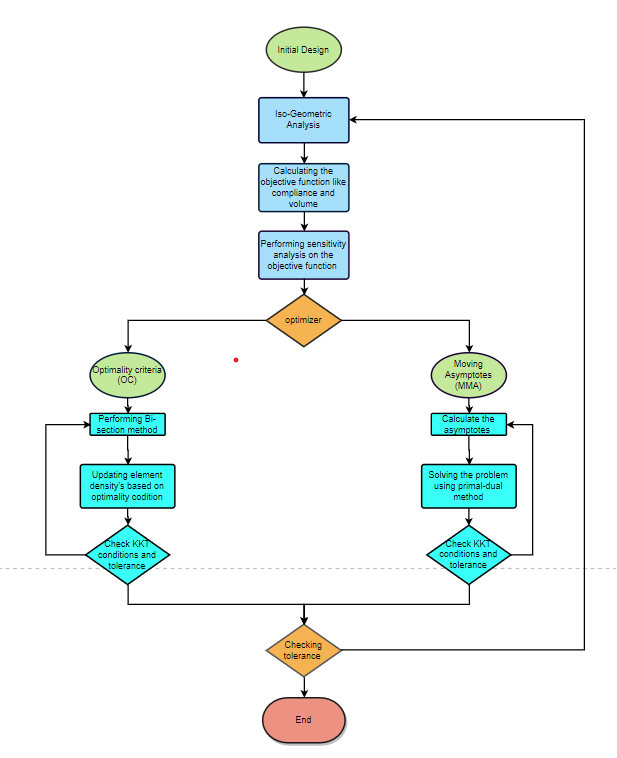
\includegraphics[width=0.65\linewidth]{topology flowchart.png}
\caption{Topology work flowchart}
\label{fig:Topology flowchart}
\end{figure}
\end{subsection}

\begin{subsection}{Post-processing}
\end{subsection}

\end{section}

%\numberwithin{equation}{section}
%this is the section on dislocation avalanches
%\input{Section_2}

%\numberwithin{equation}{section}
%this is the section on atomistic modelling on dislocations avalanches
%\input{Section_3}

%\numberwithin{equation}{section}
%this is the section is a discussion on dislocations avalanches statistics.
%\input{Section_4}

\newpage
\bibliographystyle{abbrv}
\bibliography{reference}


\end{document}